\chapter{Testbed - Prototype Implementation}
\label{chap:referenceimplementation}

As already discussed in chapter \ref{chap:introduction}, sensing a city's parking availability and thus making the parking situation more transparent would be highly beneficial for reducing traffic congestion and greenhouse gas emissions as driver's looking for parking spaces in urban areas could navigate directly to vacant parking spaces close to their destinations. In this thesis a prototype of drive-by sensing using an optical distance sensor was designed, implemented and evaluated. This chapter will discuss the test bed which was developed to acquire the necessary dataset to run the machine learning experiments.

%This chapter will describe the setup and implementation of the prototype. In particular, section \ref{sec:system_design} will discuss the overall envisioned system, the prototype car and the required sensors with their capabilities. In section \ref{sec:experiment_description_data_collection} the experimental setup will be discussed as well as the acquiring of the test dataset through test drives in the city of Linz, Austria. Finally, section \ref{sec:data_processing} will describe the preprocessing of the data, definition of the features and a short description of all used machine learning algorithms with their configurations. 
\todo{update :)}




%\section{System design}
%\label{sec:system_design}


%\begin{description}
%
%
%\item[Building a test bed] As a first step a test bed has to be built which is able to access the required sensors to record all the necessary data. A Raspberry Pi will be used as processing device because of its popularity and the many compatible sensors which work with this platform. It is connected to a LIDAR-Lite v3 sensor which continuously measures the distance to the nearest obstacle on the right side of the road. A GPS receiver will track the location of the sensing vehicle and a camera will be used to record images of the ground truth for evaluation purposes only. In section \ref{sec:system_design} the complete setup of the test bed is described as well as all the specific hard ware parts and their abilities.
%
%\item[Acquiring a dataset] As soon as the test bed is ready, the sensors should be mounted on the prototype car to be able to start recording the dataset. Test drives should be done in some selected streets in Linz, Austria with the focus of variety of the recorded situations. The test scenes should include single lane as well as multi lane streets and measurements in all streets should be done several times. Furthermore, the car should be driving as it would in regular traffic (not only in the right most lane, etc...) and the scenes should also include high and low traffic scenarios to have a high amount of diverse data. All measured distances, GPS locations and ground truth images have to be saved to files with the according timestamps to be able to evaluate the results of different approaches later on. Furthermore, using the images taken by the camera, ground truth values will be manually labelled in different classes (Parked car, free space, overtaken car, ...). A detailed description about the dataset and the ground truth tagging can be found in section \todo{ref} \ref{sec:dataset}.
%
%\item[Data processing and segmentation] As next step the measured sensor values have to be preprocessed and filtered in order for the following algorithms to work. Sensing and overflow errors as well as outliers in the measurements should be identified and removed before further processing. After the raw data has been filtered, the sensor data has to be segmented. As parking cars and other cases which should be classified consist of several sensor measurements, the corresponding sensor measurements should be grouped together and merged to segments which will be later classified. All preprocessing steps and the segmentation process are described in more detail in section \todo{ref} \ref{sec:data_processing}.
%
%\item[Classification using basic machine learning techniques] Features on the created segments are calculated (for instance length, average distance and variation of the distances) and are being used to train and evaluate several machine learning algorithms which will be compared on their performance. Furthermore, some deep learning models will also be evaluated on the raw sensor data of the segments and will be compared to common machine learning results. The results of all experiments can be found in section \todo{ref} \ref{sec:ml_results}.
%
%\item[Further improvements] \todo{todo}
%
%\end{description}









\section{Used hardware and sensor parts}
\label{sec:test_bed}

Figure \ref{fig:sensing_car} shows the sensing car and its mounted sensors. For collecting, processing and saving the sensed data a Raspberry Pi 2 Model B\footnote{\url{https://www.raspberrypi.org/products/raspberry-pi-2-model-b/}} is being used. A Raspberry Pi was chosen because of its simplicity to connect and access sensors and moreover because it is really easy to program with it as it is just a regular linux-based computer. Furthermore, the price of a Raspberry Pi is also quite low (about \euro{35}), therefore the overall cost of the system will remain low.


\begin{figure}
	\centering
	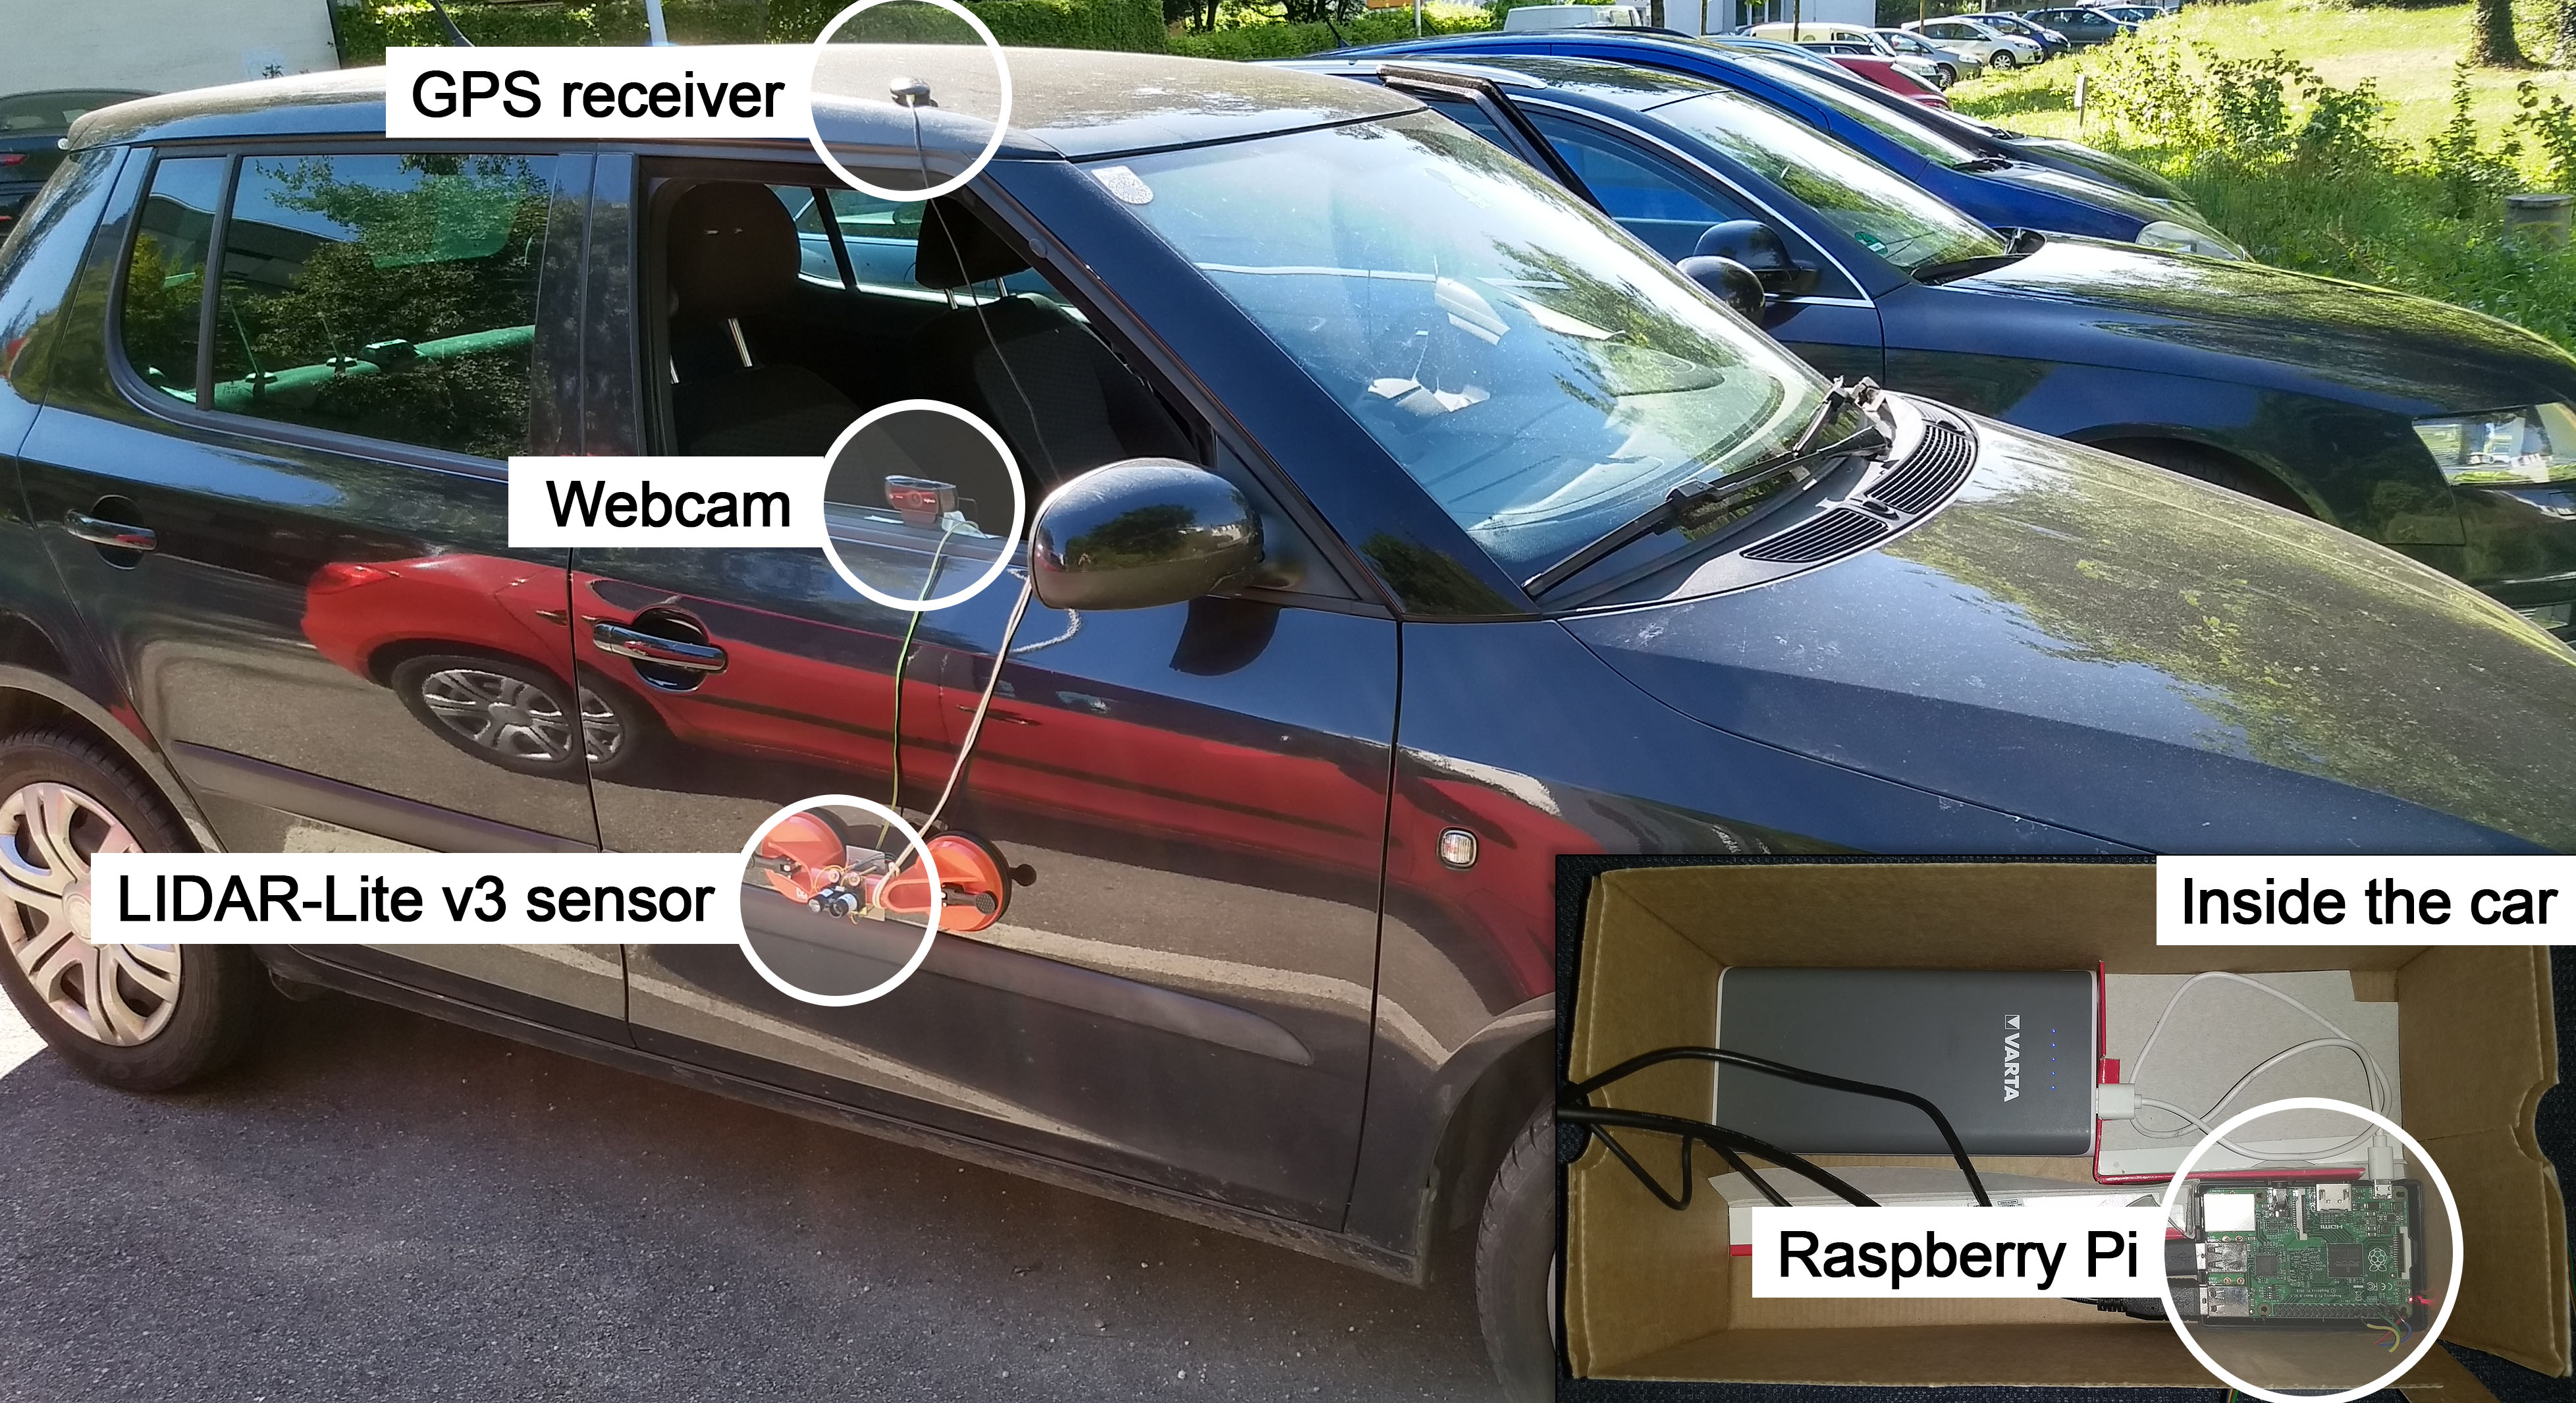
\includegraphics[width=\textwidth]{img/car.jpg}
	\caption{Prototype of the sensing car, which is composed of a LIDAR Lite v3 optical distance sensor, a GPS receiver, a camera for ground truth collection and a Raspberry Pi as processing device}
	\label{fig:sensing_car}
\end{figure}


To determine the location of the sensing vehicles while driving through the city, a Navilock USB GPS receiver\footnote{\url{http://www.navilock.de/produkte/G_61840/merkmale.html?setLanguage=en}} is being used. It can be connected to the Raspberry Pi using a USB Port and can measure the GPS location (latitude and longitude) at a rate of about 1 Hz. According to the manufacturer the acquired positions are correct in the range of 2.5 meters. The Navilock USB GPS sensor starts at a price of about \euro{50}.

For the use of a distance sensor there were two options. Either a ultrasonic range sensor could be used or an optical laser distance sensor. While ultrasonic sensors are cheap and widely used in commercial parking assistance system, they also have limitations in terms of sensing frequency (about 20 Hz) and range (a few meters). These specifications limit the use of ultrasonic sensors for using drive-by sensing on multi-lane roads or with high speed.   Due to these limitations the optical distance sensor "Lidar Lite v3\footnote{\url{https://www.sparkfun.com/products/14032}}" is being used. It measures the time of flight of an emitted laser signal which is reflected by an object in its way. The Lidar Lite v3 can measure distances from a few centimeters up to 40 meters at a frequency of 1 to 500 Hz. Furthermore, it is able to measure distances with an accuracy of about 2.5 centimeters at a distance greater than one meter. However, in comparison to ultrasonic sensors, optical sensors are more expensive. While ultrasonic sensors can be bought under \euro{10}, the Lidar Lite v3 and other comparable sensors are about \euro{150}. Table \ref{table:comparison_us_lidar} shows a comparison of the capabilities of ultrasonic sensors and the our used Lidar Lite v3 sensor. The most significant limitation is the sampling frequency. While optical laser sensors are based on the speed of light, ultrasonic sensors are based on the speed of sound, which is much slower. Therefore, also the distances between consecutive measurements varies highly from an ultrasonic to an optical laser sensor. At a speed of 50km/h and when sensing an object which is 10 meters away, a sensing vehicle would dirve about 80 cm between the measurements with an ultrasonic sensor while only driving 1 cm with an optical distance sensor.



\begin{table}

\bgroup
\def\arraystretch{1.5}
\begin{tabular}{| r || c | c |}
\hline
   & 
   \textbf{Ultrasonic Range Finder} & 
   \textbf{Lidar Lite v3} \\
%\hline
\hline
  \textbf{Costs} & 
   from about \euro{5,00} to \euro{100,00} &
   about \euro{150,00} \\
\hline
  \textbf{Sampling Frequency} & 
   up to 20 Hz &
   up to 500 Hz \\
  \textbf{(distance > 10 m)} & & \\
\hline
  \textbf{Range} & 
   2 cm - 10 m &
   30 cm - 40 m \\
\hline
  \textbf{Distance between Measurements} & 
   about 80 cm &
   about 1 cm \\
  \textbf{at 50 km/h and a distance of 10 m} & & \\
\hline

\end{tabular}
\egroup

\caption{Comparison of ultrasonic sensors and optical (LiDAR) sensors}
\label{table:comparison_us_lidar}
\end{table}


%\begin{table}
%
%\bgroup
%\def\arraystretch{1.5}
%\begin{tabular}{| r || c | c |}
%\hline
%   & 
%   \textbf{Sampling Frequency} & 
%   \textbf{Costs per Sensor} \\
%%\hline
%\hline
%  \textbf{Lidar Lite v3} & 
%   ~200 measurements/s &
%   \euro{169,00} \\
%\hline
%  \textbf{Navilock USB} & 
%   ~1 measurement/s &
%   \euro{74,90} \\
%   \textbf{GPS receiver} & & \\
%\hline
%
%\end{tabular}
%\egroup
%
%\caption{The used sensors}
%\label{table:sensors_capabilities}
%\end{table}


\section{Collecting Sensor Measurements}

Figure \ref{fig:sample_sensor_trace} shows a sample sensor trace :)

\begin{figure}
	\centering
	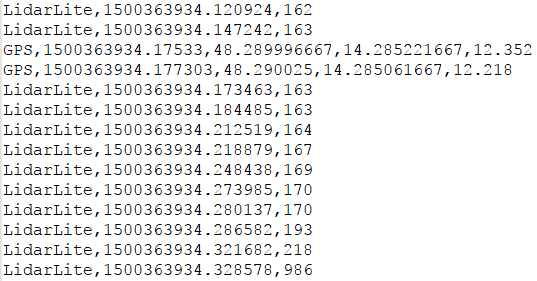
\includegraphics{img/sample-sensor-trace.PNG}
	\caption{Sample of the collected sensor trace}
	\label{fig:sample_sensor_trace}
\end{figure}







\chapter{Data Processing and Machine Learning Approaches}

\section{Experiment description and data collection}
\label{sec:experiment_description_data_collection}
- Description of experiments (scenarios we are interested in: parking car, etc.)
- Data set derived (raw data, size, etc.)
- Map data and camera ground truth data

\begin{figure}
	\centering
	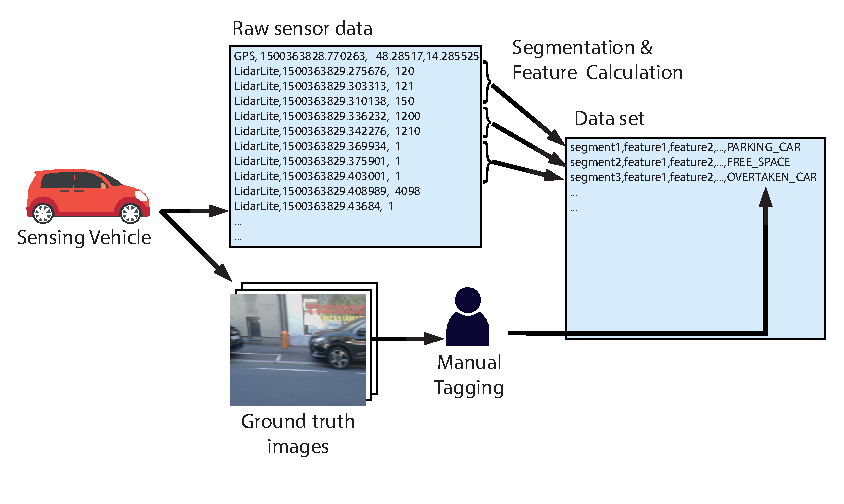
\includegraphics[width=\textwidth]{img/obtaining-dataset-architecture.eps}
	\caption{Steps to obtain the dataset from the raw sensor measurements and ground truth recordings}
	\label{fig:dataset_architecture}
\end{figure}

\section{Data processing}
\label{sec:data_processing}
- Preprocessing, feature definition ...
- Traditional ML Algorithms (incl. a short description of each algorithm and configuration options)
- Deep Learning